\documentclass[12pt,a4paper]{article}

% --- Настройка языка и шрифтов для LuaLaTeX ---
\usepackage{fontspec}
\defaultfontfeatures{Ligatures=TeX,Scale=MatchLowercase}

\setmainfont{Alice-Regular}[
    Path=font/,
    Extension=.ttf,
    BoldFont = Alice-Regular,
    ItalicFont = Alice-Regular,
    BoldItalicFont = Alice-Regular,
    BoldFeatures = {FakeBold=1.6},
    ItalicFeatures = {FakeSlant=0.2},
    BoldItalicFeatures = {FakeBold=1.6,FakeSlant=0.2}
]

\newfontfamily\cyrillicfont{Alice-Regular}[
    Path=font/,
    Extension=.ttf,
    BoldFont = Alice-Regular,
    ItalicFont = Alice-Regular,
    BoldItalicFont = Alice-Regular,
    BoldFeatures = {FakeBold=1.6},
    ItalicFeatures = {FakeSlant=0.2},
    BoldItalicFeatures = {FakeBold=1.6,FakeSlant=0.2}
]

\usepackage{polyglossia}
\setmainlanguage{russian}
\setsansfont{TeX Gyre Heros}
\setmonofont{TeX Gyre Cursor}

\usepackage{xcolor}                             % Цвета
\usepackage{graphicx}                           % Графика
\usepackage[protrusion=false]{microtype}        % Микротипографика
\usepackage{amsmath, amsfonts, amssymb, amsthm} % Математика
\usepackage{braket}                             % Braket нотация для квантовой механики
\usepackage{unicode-math}                       % Современный пакет для математики в LuaLaTeX
\usepackage{longtable}                          % Таблицы с разрывом страниц
\usepackage{tikz}                               % Рисование
\usepackage[europeanresistors]{circuitikz}      % Рисование электрических схем в европейском стиле
\usepackage{listings}                           % Для отображения кода
\usepackage{tabularx}                           % Для таблиц во всю ширину
\usepackage{array}                              % Для расширенных возможностей таблиц
\usepackage{multirow}                           % Для объединения ячеек таблиц
\usepackage{float}                              % Для точного позиционирования фигур
\usepackage{pgfplots}                           % Для построения графиков
\usepackage{caption}                            % Для настройки подписей к рисункам и таблицам
\usepackage{xfp}                                % Для вычислений в LaTeX
\usepackage{luacode}                            % Для выполнения Lua-кода в документе
\pgfplotsset{compat=1.18}
\usepackage{textcomp}                          % Для знака номера (\textnumero)
\usepackage{makecell}                          % Для переносов строк внутри ячеек таблиц
\usepackage[a4paper,left=20mm,right=20mm,top=20mm,bottom=20mm]{geometry}

\usetikzlibrary{arrows.meta}

% --- Колонтитулы ---
\usepackage{fancyhdr}
\pagestyle{fancy}
\fancyhf{}

\renewcommand{\headrulewidth}{0.4pt}
\renewcommand{\footrulewidth}{0.4pt}
\renewcommand\lstlistingname{Исходный код}

\lstdefinestyle{main}{
	backgroundcolor=\color{gray!8},
	commentstyle=\color{green!50!black},
	keywordstyle=\color{blue!80!black},
	numberstyle=\small\color{darkgray},
	stringstyle=\rmfamily\color{orange!90!black},
	basicstyle=\ttfamily\small,
	breakatwhitespace=false,
	breaklines=true,
	keepspaces=true,
	numbers=left,
	numbersep=8pt,
	showspaces=false,
	showstringspaces=false,
	showtabs=false,
	tabsize=4
}

\lstset{style=main}

\newcolumntype{C}{>{\centering\arraybackslash}X}
\newcolumntype{Y}[1]{>{\centering\arraybackslash}p{#1}}
\renewcommand{\arraystretch}{1.25}

% =========================================================
%         СЛУЖЕБНЫЕ КОМАНДЫ ДЛЯ ВЫЧИСЛЕНИЙ
% =========================================================
\newcommand{\CalcZero} [1]{\fpeval{round((#1),0)}}
\newcommand{\CalcOne}  [1]{\fpeval{round((#1),1)}}
\newcommand{\CalcTwo}  [1]{\fpeval{round((#1),2)}}
\newcommand{\CalcThree}[1]{\fpeval{round((#1),3)}}
\newcommand{\CalcFour} [1]{\fpeval{round((#1),4)}}
\newcommand{\CalcFive} [1]{\fpeval{round((#1),5)}}

\begin{luacode*}
-- Данные для задания 1

-- Первый столбец - расстояние в см,
-- Следующие 5 столбцов - результаты измерений в мс (5 раз подряд для каждого расстояния)
-- Масштаб осциллографа задается в секундах на деление
E1 = {
  {D = 20,  X = {1.1897, 1.2167, 1.2167, 1.2166, 1.2406}, KT = 0.001},
  {D = 25,  X = {1.5701, 1.5973, 1.5702, 1.7111, 1.7108}, KT = 0.001},
  {D = 30,  X = {2.0438, 1.9900, 1.9898, 1.9627, 1.9629}, KT = 0.005},
  {D = 35,  X = {2.1964, 2.1964, 2.1696, 2.1696, 2.1933}, KT = 0.005},
  {D = 40,  X = {2.4421, 2.3971, 2.3971, 2.3943, 2.4240}, KT = 0.005},
  {D = 45,  X = {2.7268, 2.7178, 2.7181, 2.7688, 2.7690}, KT = 0.005},
  {D = 50,  X = {2.9339, 3.0092, 2.9549, 2.9762, 2.9526}, KT = 0.005},
  {D = 55,  X = {3.2695, 3.2400, 3.2362, 3.2370, 3.2275}, KT = 0.005},
  {D = 60,  X = {3.5959, 3.6441, 3.5931, 3.6682, 3.6954}, KT = 0.005},
  {D = 65,  X = {3.7939, 3.7938, 3.8176, 3.8418, 3.7937}, KT = 0.005},
  {D = 70,  X = {4.0875, 4.0844, 4.0847, 4.1086, 4.1058}, KT = 0.005},
  {D = 75,  X = {4.4143, 4.3867, 4.4349, 4.4318, 4.4294}, KT = 0.005},
  {D = 80,  X = {4.7438, 4.7198, 4.7197, 4.6420, 4.6416}, KT = 0.005},
  {D = 85,  X = {4.8766, 4.8849, 4.9361, 4.8892, 4.8826}, KT = 0.005},
  {D = 90,  X = {5.2294, 5.2269, 5.2240, 5.2504, 5.2293}, KT = 0.005},
  {D = 95,  X = {5.5561, 5.5327, 5.5144, 5.5411, 5.5085}, KT = 0.005},
  {D = 100, X = {5.8468, 5.7599, 5.8113, 5.7721, 5.7934}, KT = 0.005},
}

-- Данные для задания 2

-- Первый столбец - напряжение питания схемы в В,
-- Второй столбец - ток потребления схемы в А,
-- Третий столбец - измеренное напряжение в точке A в В,
-- Четвертый столбец - измеренное напряжение в точке B в В,
E2 = {
  {U = 0.999, I = 0.001, UA = 0.73341, UB = 0.42816},
  {U = 1.999, I = 0.001, UA = 1.4477,  UB = 0.84905},
  {U = 2.999, I = 0.001, UA = 2.1654,  UB = 1.2795},
  {U = 4.000, I = 0.001, UA = 2.8772,  UB = 1.7035},
  {U = 4.999, I = 0.002, UA = 3.6071,  UB = 2.1253},
  {U = 5.998, I = 0.002, UA = 4.3124,  UB = 2.5490},
  {U = 6.999, I = 0.003, UA = 5.0838,  UB = 3.0494},
  {U = 7.998, I = 0.004, UA = 5.8182,  UB = 3.4798},
  {U = 8.998, I = 0.005, UA = 6.5513,  UB = 3.8824},
  {U = 9.999, I = 0.006, UA = 7.2567,  UB = 4.3022},
}

-- безопасная версия value_with_mantice
local function round_fallback(x)
  if x >= 0 then return math.floor(x + 0.5) else return math.ceil(x - 0.5) end
end
local round = math.round or round_fallback

-- Функция для форматирования числа в виде мантиссы и экспоненты
-- value - число для форматирования
-- precision - количество значимых цифр в мантиссе
-- shift - сдвиг порядка для экспоненты
-- scale - дополнительный масштаб для мантиссы (например, для перевода в другую единицу измерения)
function value_with_mantice(value, precision, shift, scale)
  precision = precision or 5
  shift = shift or 0
  scale = scale or 0

  if value == nil or value ~= value then
    return "\\fpeval{0}"
  end
  if value == 0 then
    return "\\fpeval{0}"
  end

  local sign = ""
  if value < 0 then
    sign = "-"
    value = math.abs(value)
  end

  local logv = math.log10(value)
  if not (logv == logv) then -- проверка на NaN
    return "\\fpeval{0}"
  end

  local floorlog = math.floor(logv)
  local mantissa = round(value * 10^(precision - 1 - floorlog)) * 10^(-(precision - 1) + shift - scale)
  local exponent = floorlog - shift

  if exponent == 0 then
    return sign .. "\\fpeval{" .. mantissa .. "}"
  else
    return sign .. "\\fpeval{" .. mantissa .. "} \\cdot 10^{" .. exponent .. "}"
  end
end

function mean(t)
  local s = 0
  for _, v in ipairs(t) do s = s + v end
  return s / #t
end

function stdev(t)
  local m = mean(t)
  local s = 0
  for _, v in ipairs(t) do s = s + (v - m)^2 end
  return math.sqrt(s / (#t - 1))
end

function median(t)
  local u = {}
  for i, v in ipairs(t) do u[i] = v end
  table.sort(u)
  local n = #u
  if n % 2 == 1 then
    return u[(n + 1) / 2]
  else
    return (u[n / 2] + u[n / 2 + 1]) / 2
  end
end

function raw_number(v)
  return string.format("%.10g", v)
end

function print_value(value, precision, shift, scale)
  tex.sprint(value_with_mantice(value, precision, shift, scale))
end

-- Вычисления для задания 1
for _, row in ipairs(E1) do
  row.Xmean = mean(row.X)
  row.S = stdev(row.X)
end

function compute_e1()
  local xs, ys = {}, {}
  for _, row in ipairs(E1) do
    for _, x in ipairs(row.X) do
      table.insert(xs, row.D)
      table.insert(ys, x)
    end
  end

  local n = #xs
  local sx, sy, sxx, sxy, syy = 0, 0, 0, 0, 0
  for i = 1, n do
    sx = sx + xs[i]
    sy = sy + ys[i]
    sxx = sxx + xs[i]^2
    sxy = sxy + xs[i] * ys[i]
    syy = syy + ys[i]^2
  end

  local det = n * sxx - sx^2
  local b1 = (n * sxy - sx * sy) / det
  local b0 = (sy - b1 * sx) / n

  local ss_res = 0
  local ymean = sy / n
  local ss_tot = 0
  for i = 1, n do
    local yhat = b0 + b1 * xs[i]
    ss_res = ss_res + (ys[i] - yhat)^2
    ss_tot = ss_tot + (ys[i] - ymean)^2
  end

  local m = 2
  local S2 = ss_res / (n - m)
  local V00 = S2 * sxx / det
  local V11 = S2 * n / det
  local t = 1.98896 -- t_{0.975,83}
  local R2 = 1 - ss_res / ss_tot

  local median_centers = {}
  local group_limits = {{1,6}, {7,12}, {13,17}}
  for g, lim in ipairs(group_limits) do
    local dx, yy = {}, {}
    for i = lim[1], lim[2] do
      for _, val in ipairs(E1[i].X) do
        table.insert(dx, E1[i].D)
        table.insert(yy, val)
      end
    end
    median_centers[g] = {D = median(dx), X = median(yy)}
  end

  return {
    n = n,
    m = m,
    sx = sx,
    sy = sy,
    sxx = sxx,
    sxy = sxy,
    syy = syy,
    det = det,
    ss_res = ss_res,
    ss_tot = ss_tot,
    b0 = b0,
    b1 = b1,
    S2 = S2,
    S = math.sqrt(S2),
    V00 = V00,
    V11 = V11,
    db0 = t * math.sqrt(V00),
    db1 = t * math.sqrt(V11),
    r = (n * sxy - sx * sy) / math.sqrt((n * sxx - sx^2) * (n * syy - sy^2)),
    R2 = R2,
    rho = math.sqrt(R2),
    t = t,
    df = n - m,
    median_centers = median_centers,
  }
end

E1FIT = compute_e1()

-- Вычисления для задания 2
function compute_e2()
  local sumI2 = 0
  local sumIR1, sumIR2, sumIR3 = 0, 0, 0
  local equations = {}

  for _, row in ipairs(E2) do
    local y1 = row.U - row.UA
    local y2 = row.UA - row.UB
    local y3 = row.UB

    sumI2 = sumI2 + row.I^2
    sumIR1 = sumIR1 + row.I * y1
    sumIR2 = sumIR2 + row.I * y2
    sumIR3 = sumIR3 + row.I * y3

    table.insert(equations, {R = 1, I = row.I, y = y1})
    table.insert(equations, {R = 2, I = row.I, y = y2})
    table.insert(equations, {R = 3, I = row.I, y = y3})
  end

  local R1 = sumIR1 / sumI2
  local R2 = sumIR2 / sumI2
  local R3 = sumIR3 / sumI2
  local R = {R1, R2, R3}

  local ss = 0
  for _, eq in ipairs(equations) do
    ss = ss + (eq.y - eq.I * R[eq.R])^2
  end

  local n = #equations
  local m = 3
  local S2 = ss / (n - m)
  local V = S2 / sumI2
  local t = 2.05183 -- t_{0.975,27}

  return {
    n = n,
    m = m,
    sumI2 = sumI2,
    sumIR1 = sumIR1,
    sumIR2 = sumIR2,
    sumIR3 = sumIR3,
    ss = ss,
    R1 = R1,
    R2 = R2,
    R3 = R3,
    V = V,
    dR1 = t * math.sqrt(V),
    dR2 = t * math.sqrt(V),
    dR3 = t * math.sqrt(V),
    S2 = S2,
    S = math.sqrt(S2),
    t = t,
    df = n - m,
  }
end

E2FIT = compute_e2()

function print_e1_protocol()
  for i, row in ipairs(E1) do
    tex.sprint("$" .. i .. "$ & \\centering $" .. row.D .. "$ & \\centering $" .. value_with_mantice(row.KT, 3, -3, -3) .. "$ & ")
    for j = 1, 4 do
      tex.sprint("$" .. value_with_mantice(row.X[j], 5, 0, 0) .. "$ & ")
    end
    tex.sprint("$" .. value_with_mantice(row.X[5], 5, 0, 0) .. "$ \\\\ \\hline")
  end
end

function print_e1_protocol1()
  for i, row in ipairs(E1) do
    tex.sprint("$" .. i .. "$ & \\centering $" .. row.D .. "$ & \\centering $" .. value_with_mantice(row.KT, 3, -3, -3) .. "$ & $" .. value_with_mantice(row.Xmean, 5, 0, 0) .. "$ & $" .. value_with_mantice(row.S, 3, -2, 0) .. "$ \\\\ \\hline")
  end
end

function print_e2_protocol()
  for i, row in ipairs(E2) do
    tex.sprint("$" .. i .. "$ & $" .. row.U .. "$ & $" .. value_with_mantice(row.I, 4, -3, 0) .. "$ & $" .. row.UA .. "$ & $" .. row.UB .. "$ \\\\ \\hline")
  end
end

function print_e1_all_points()
  for _, row in ipairs(E1) do
    for _, val in ipairs(row.X) do
      tex.sprint("(" .. raw_number(row.D) .. "," .. raw_number(val) .. ")")
    end
  end
end

function print_e1_mean_points()
  for _, row in ipairs(E1) do
    tex.sprint("(" .. raw_number(row.D) .. "," .. raw_number(row.Xmean) .. ")")
  end
end

function print_e1_median_centers()
  for i, c in ipairs(E1FIT.median_centers) do
    tex.sprint("$" .. i .. "$ & $" .. value_with_mantice(c.D, 4, 1, 0) .. "$ & $" .. value_with_mantice(c.X, 5, 0, 0) .. "$ \\\\ \\hline")
  end
end

function print_e1_median_points()
  for _, c in ipairs(E1FIT.median_centers) do
    tex.sprint("(" .. raw_number(c.D) .. "," .. raw_number(c.X) .. ")")
  end
end

function print_e2_drop_table()
  for i, row in ipairs(E2) do
    local UR1 = row.U - row.UA
    local UR2 = row.UA - row.UB
    local UR3 = row.UB
    tex.sprint("$" .. i .. "$ & $" .. UR1 .. "$ & $" .. UR2 .. "$ & $" .. UR3 .. "$ \\\\ \\hline")
  end
end

function print_e2_ur_points(k)
  for _, row in ipairs(E2) do
    local y = 0
    if k == 1 then
      y = row.U - row.UA
    elseif k == 2 then
      y = row.UA - row.UB
    else
      y = row.UB
    end
    tex.sprint("(" .. raw_number(row.I * 1000) .. "," .. raw_number(y) .. ")")
  end
end
\end{luacode*}

% ---------------------------------------------------------
% ОБЩИЕ ДАННЫЕ
% ---------------------------------------------------------
\def\VariantN{4}                                 % Номер варианта
\def\LabNumber{4}                                % Номер лабораторной работы
\def\Discipline{Метрология}                      % Название дисциплины
\def\LabTitle{Совместные и совокупные измерения} % Название лабораторной работы

\title{
	МИНОБРНАУКИ РОССИИ

	федеральное государственное автономное образовательное учреждение

	высшего образования

	«Национальный исследовательский университет
	«Московский институт электронной техники»
	\vspace{2em}
}
\author{
}
\date{}

\begin{document}

\maketitle
\thispagestyle{fancy}

\begin{center}
\Large Отчёт по Лабораторной работе $\LabNumber$\\
по дисциплине «\Discipline»\\
«\LabTitle»
\end{center}

\begin{center}
\Large Вариант \VariantN
\end{center}

\vspace{12em}

\begin{flushright}
	Выполнили студенты группы ЭН-$25$\\
	Андреев И. А.\\
	Анисимов А. С.\\
  и ЭН-$21$ \\ 
  Рыжов Р. Р.\\
	Проверил преподаватель\\
	Туринцев К. А.
\end{flushright}

\cfoot{Москва 2026}

\pagebreak

\fancyhead[L]{\LabTitle}
\fancyhead[R]{\Discipline}
\fancyfoot[C]{\thepage}


\pagebreak
\fancyhead[L]{Оглавление}
\fancyhead[R]{\LabTitle}
\fancyfoot[C]{\thepage}
\tableofcontents
\pagebreak

\fancyhead[L]{Теория}
\fancyhead[R]{\LabTitle}

\begin{center}
\Large\textbf{Лабораторная работа $\LabNumber$}
\end{center}

\begin{center}
\LARGE\textbf{\LabTitle}
\end{center}

\large\textbf{\textit{Цель работы}:} постановка многократных совместных и совокуп-
ных измерений и оценка действительных значений измеряемых величин
с последующей оценкой погрешностей данных измерений.

\large\textbf{\textit{Необходимое оборудование}:} цифровой мультиметр
(\textbf{Rigol DM$3058$}), генератор сигналов (\textbf{Rigol DG$1022$Z}),
цифровой осциллограф (\textbf{Rigol MSO$5102$}), источник питания (\textbf{Rigol DP$800$A}), макетная плата, кабели,
перемычки, щупы.

\normalsize
\fancyhead[L]{Теория}
\section{Теоретические сведения}

Совместные измерения – проводимые одновременно измерения
двух или нескольких неодноименных величин для определения зависимости между ними.

В отличие от совместных, совокупные измерения – проводимые одновременно измерения
нескольких одноименных величин, при которых
искомые значения величин определяют путем решения системы уравнений, получаемых при
измерениях этих величин в разных сочетаниях.
Иными словами, совокупные измерения обычно предусматривают
несколько измерительных уравнений для одной и той же физической
величины (или величин одного типа), что позволяет вычислить ее значение с повышенной
точностью.

Совместные и совокупные измерения, как правило, организуют таким образом,
что число независимых уравнений, связывающих измеряемые величины,
превышает число определяемых величин. Это означает,
что экспериментальные данные избыточны – ситуация, при которой
нельзя найти единственное решение простым прямым методом, и возникает
необходимость в аппроксимации и статистической обработке
данных.

\subsection{Постановка измерительного эксперимента и сбор данных}

В совместных измерениях одновременно получают значения нескольких
неодноименных физических величин. В данной лабораторной работе одна
из величин задается непосредственно в ходе эксперимента – расстояние
$D$ от ультразвукового дальномера до преграды, а другая измеряется
по выходному сигналу дальномера с помощью осциллографа. Измерение
повторяется несколько раз для каждого установленного расстояния, поэтому
для одной и той же точки градуировочной характеристики получается выборка
значений $X_{i1}, X_{i2}, \ldots, X_{i5}$.

Поскольку экспериментальные значения содержат случайные отклонения,
каждая точка на графике рассматривается не как абсолютно точное значение,
а как результат многократного измерения. Для расстояния $D_i$ среднее
значение выходного параметра дальномера вычисляется по формуле \eqref{eq:mean-x}:
\begin{equation}
\overline{X}_i = \frac{1}{n_i}\sum\limits_{j = 1}^{n_i} X_{ij}
\tag{1.1}
\label{eq:mean-x}
\end{equation}
а выборочное среднеквадратическое отклонение вычисляется по формуле \eqref{eq:std-x}:
\begin{equation}
S_{X_i} = \sqrt{\frac{1}{n_i - 1}\sum\limits_{j = 1}^{n_i}\left(X_{ij} - \overline{X}_i\right)^2}
\tag{1.2}
\label{eq:std-x}
\end{equation}

При совокупных измерениях одновременно измеряются одноименные
величины в разных сочетаниях. В этой работе таким образом оцениваются
сопротивления $R_1$, $R_2$ и $R_3$: измеряются напряжение питания цепи,
ток потребления и напряжения в точках A и B, после чего составляется
переопределенная система уравнений относительно неизвестных сопротивлений.

\subsection{Выбор вида математической модели}

Перед вычислением коэффициентов необходимо выбрать вид условной функции,
которая будет связывать независимую величину $D$ и выходной параметр
дальномера $X$. Если физическая природа измерительного преобразователя
известна заранее, вид зависимости выбирается на основании этой природы.
Для ультразвукового дальномера длительность выходного импульса связана
со временем распространения акустической волны до преграды и обратно,
поэтому ожидается зависимость, близкая к линейной.

При отсутствии полной уверенности в виде модели используют графические
приемы предварительного анализа. Метод контура состоит в том, что область
разброса экспериментальных точек ограничивают внешним контуром и по форме
этого контура судят о возможной зависимости. Если контур вытянут вдоль
прямой линии, выбирается линейная модель; если наблюдается изгиб, рассматривают
полиномиальную, степенную или другую нелинейную модель.

Метод медианных центров состоит в разбиении экспериментальных точек на
несколько групп по возрастанию независимой переменной. Для каждой группы
находят медиану по оси $D$ и медиану по оси $X$, после чего по взаимному
расположению медианных центров выбирают простейший подходящий вид модели.
В данной работе медианные центры лежат почти на одной прямой, поэтому
принимается линейная модель \eqref{eq:linear-model}:
\begin{equation}
X = b_0 + b_1D
\tag{2}
\label{eq:linear-model}
\end{equation}

\subsection{Подбор аппроксимирующей функции}

После выбора вида модели необходимо определить ее коэффициенты.
В общем случае для совместных измерений используется аппроксимирующая
функция
\begin{equation*}
y = f(x, \mathbf{a})
\end{equation*}
где $\mathbf{a}$ – вектор неизвестных параметров. Если функция линейна по
параметрам, задача может быть решена методом наименьших квадратов.

Для полиномиальной модели степени $m$
\begin{equation*}
y = b_0 + b_1x + a_2x^2 + \ldots + a_mx^m
\end{equation*}
матрица наблюдений имеет вид
\begin{equation*}
X =
\begin{pmatrix}
1 & x_1 & x_1^2 & \ldots & x_1^m\\
1 & x_2 & x_2^2 & \ldots & x_2^m\\
\ldots & \ldots & \ldots & \ldots & \ldots\\
1 & x_n & x_n^2 & \ldots & x_n^m
\end{pmatrix}
\qquad
\mathbf{y} =
\begin{pmatrix}
y_1\\y_2\\\ldots\\y_n
\end{pmatrix}
\end{equation*}

Если экспериментально наблюдается степенная зависимость
\begin{equation*}
y = bx^a
\end{equation*}
то ее можно привести к линейному виду логарифмированием:
\begin{equation*}
\ln y = \ln b + a\ln x
\end{equation*}
Гиперболическую или дробно-рациональную зависимость также часто упрощают
заменой переменных, например переходом к $1/x$ или $1/y$.
В данной работе по результатам графического анализа используется линейная
аппроксимация, так как усложнение модели не требуется.

\subsection{Расчет по экспериментальным данным параметров
выбранной аппроксимирующей функции}

Пусть имеется $n$ экспериментальных точек и выбрана модель
\begin{equation*}
y_i = f(x_i, \mathbf{a}) + \nu_i
\end{equation*}
где $\nu_i$ – невязка $i$-го измерения. Метод наименьших квадратов требует
найти такие значения параметров, чтобы сумма квадратов невязок была минимальной:
\begin{equation*}
F(\mathbf{a}) = \sum\limits_{i = 1}^{n}\left(y_i - f(x_i, \mathbf{a})\right)^2 \rightarrow \min
\end{equation*}

Для модели, линейной по параметрам, решение записывается в матричной форме по формуле 
\begin{equation}
X^TX\mathbf{a} = X^T\mathbf{y}
\tag{4}
\label{eq:mnk-solution}
\end{equation}

Для линейной модели \eqref{eq:linear-model} коэффициенты можно вычислить
через суммы экспериментальных значений по формулам \eqref{eq:e1-b1} и \eqref{eq:e1-b0}:
\begin{equation}
b_1 =
\frac{n\sum\limits_{i = 1}^{n}D_iX_i - \sum\limits_{i = 1}^{n}D_i\sum\limits_{i = 1}^{n}X_i}
{n\sum\limits_{i = 1}^{n}D_i^2 - \left(\sum\limits_{i = 1}^{n}D_i\right)^2}
\tag{4.1}
\label{eq:e1-b1}
\end{equation}
\begin{equation}
b_0 =
\frac{\sum\limits_{i = 1}^{n}X_i - b_1\sum\limits_{i = 1}^{n}D_i}{n}
\tag{4.2}
\label{eq:e1-b0}
\end{equation}

Для линейной зависимости $X = b_0 + b_1D$ коэффициенты можно вычислять
по тем же нормальным уравнениям. В этой работе вектор неизвестных параметров
имеет вид
\begin{equation*}
\mathbf{b} =
\begin{pmatrix}
b_0\\b_1
\end{pmatrix}
\end{equation*}
а матрица наблюдений содержит первый столбец из единиц и второй столбец
из расстояний $D_i$.

\subsection{Оценка величин резисторов $R_1$, $R_2$ и $R_3$ соединённых звездой}

В эксперименте с совокупными измерениями используются показания напряжения
питания $U_{\text{пит}}$, тока потребления $I$, напряжения в точке A $U_A$
и напряжения в точке B $U_B$. Для последовательных падений напряжения на
резисторах справедливы уравнения \eqref{eq:resistor-equations}:
\begin{equation}
\begin{cases}
I_iR_1 = U_{\text{пит},i} - U_{A,i}\\
I_iR_2 = U_{A,i} - U_{B,i}\\
I_iR_3 = U_{B,i}
\end{cases}
\tag{5.1}
\label{eq:resistor-equations}
\end{equation}

Для всех строк протокола эти уравнения объединяются в переопределенную
систему
\begin{equation*}
\mathbf{y} = X\mathbf{R}
\qquad
\mathbf{R} =
\begin{pmatrix}
R_1\\R_2\\R_3
\end{pmatrix}
\end{equation*}
где вектор $\mathbf{y}$ содержит измеренные падения напряжений
$U_{\text{пит}} - U_A$, $U_A - U_B$, $U_B$, а матрица $X$ содержит
соответствующие коэффициенты при $R_1$, $R_2$, $R_3$
\begin{equation*}
X =
\begin{pmatrix}
I_1 & 0 & 0\\
0 & I_1 & 0\\
0 & 0 & I_1\\
I_2 & 0 & 0\\
0 & I_2 & 0\\
0 & 0 & I_2\\
\ldots & \ldots & \ldots
\end{pmatrix}
\end{equation*}

Так как число уравнений больше числа неизвестных, решение находится методом
наименьших квадратов по формуле
\begin{equation}
\mathbf{R} = \left(X^TX\right)^{-1}X^T\mathbf{y}
\tag{5.2}
\label{eq:mnk-resistors}
\end{equation}

Для примененной схемы матрицы коэффициентов формула \eqref{eq:mnk-resistors}
сводится к независимому вычислению каждого сопротивления по формуле \eqref{eq:resistor-simple}:
\begin{equation}
R_j =
\frac{\sum\limits_{i = 1}^{n} I_i U_{R_j,i}}
{\sum\limits_{i = 1}^{n} I_i^2}
\qquad j = 1,2,3
\tag{5.3}
\label{eq:resistor-simple}
\end{equation}

\subsection{Оценка качества аппроксимации}

Качество аппроксимации удобно оценивать через коэффициент корреляции
Пирсона и коэффициент множественной корреляции. Коэффициент корреляции
Пирсона для двух величин $x$ и $y$ вычисляется по формуле 
\begin{equation}
\rho_{xy} =
\frac{\sum\limits_{i = 1}^{n}(x_i - \overline{x})(y_i - \overline{y})}
{\sqrt{\sum\limits_{i = 1}^{n}(x_i - \overline{x})^2\sum\limits_{i = 1}^{n}(y_i - \overline{y})^2}}
\tag{6.1}
\label{eq:pearson}
\end{equation}

Значение $|\rho_{xy}|$, близкое к единице, указывает на сильную линейную
зависимость между величинами. Для оценки соответствия расчетных значений
$\widehat{y}_i$ экспериментальным значениям $y_i$ используется коэффициент
детерминации по формуле 
\begin{equation}
R^2 = 1 - \frac{\sum\limits_{i = 1}^{n}(y_i - \widehat{y}_i)^2}
{\sum\limits_{i = 1}^{n}(y_i - \overline{y})^2}
\tag{6.2}
\label{eq:determination}
\end{equation}
и коэффициент множественной корреляции
\begin{equation*}
\rho_{y\widehat{y}} = \sqrt{R^2}
\tag{6.3}
\label{eq:multiple-correlation}
\end{equation*}

Если коэффициенты корреляции по модулю превышают $0,95$, то условная
функция считается подобранной корректно для инженерной обработки результатов.

\subsection{Результаты совместных измерений
и их доверительная оценка}

После нахождения коэффициентов модели анализируют невязки
\begin{equation*}
\nu_i = y_i - \widehat{y}_i
\end{equation*}
Остаточная выборочная дисперсия погрешностей определяется по формуле
\begin{equation}
S^2 = \frac{\sum\limits_{i = 1}^{n}\left(y_i - \widehat{y}_i\right)^2}{n - m}
\tag{7.1}
\label{eq:residual-variance}
\end{equation}
где $n$ – число экспериментальных значений, а $m$ – число оцениваемых
параметров модели.

Ковариационная матрица оценок коэффициентов модели вычисляется по формуле
\begin{equation}
V = S^2\left(X^TX\right)^{-1}
\tag{7.2}
\label{eq:covariance}
\end{equation}
Для линейной модели \eqref{eq:linear-model} диагональные элементы этой матрицы
удобно записать по формуле \eqref{eq:e1-v00}:
\begin{equation}
V_{00} = S^2\frac{\sum\limits_{i = 1}^{n}D_i^2}{\Delta}
\qquad
V_{11} = S^2\frac{n}{\Delta}
\qquad
\Delta = n\sum\limits_{i = 1}^{n}D_i^2 -
\left(\sum\limits_{i = 1}^{n}D_i\right)^2
\tag{7.2.1}
\label{eq:e1-v00}
\end{equation}
\begin{equation}
\Delta a_j = t_{q;\,\nu}\sqrt{V_{jj}}
\tag{7.2.2}
\label{eq:delta-coeff}
\end{equation}
На главной диагонали матрицы $V$ находятся оценки дисперсий коэффициентов.
При предположении нормального закона распределения случайных погрешностей
доверительные границы коэффициентов при доверительной вероятности $0,95$
записываются по формуле
\begin{equation}
a_j \pm t_{q;\,n-2}\sqrt{V_{jj}}
\tag{7.3}
\label{eq:confidence-coeff}
\end{equation}

\pagebreak

\begin{center}
\LARGE{\textbf{Выполнение лабораторной работы и расчетно-графическая часть}}
\end{center}

\fancyhead[L]{Задание $1$}
\section{Совместное измерение расстояния от дальномера до преграды и выходного параметра дальномера}

\subsection{Схема и протокол совместных измерений}

Генератор сигналов использовался для запуска измерения,
источник питания задавал рабочее напряжение дальномера, а осциллографом
измерялся выходной параметр дальномера $X$ в миллисекундах. Для каждого расстояния $D$ 
от дальномера до преграды проводилось по пять измерений.
\begin{figure}[H]
	\centering
	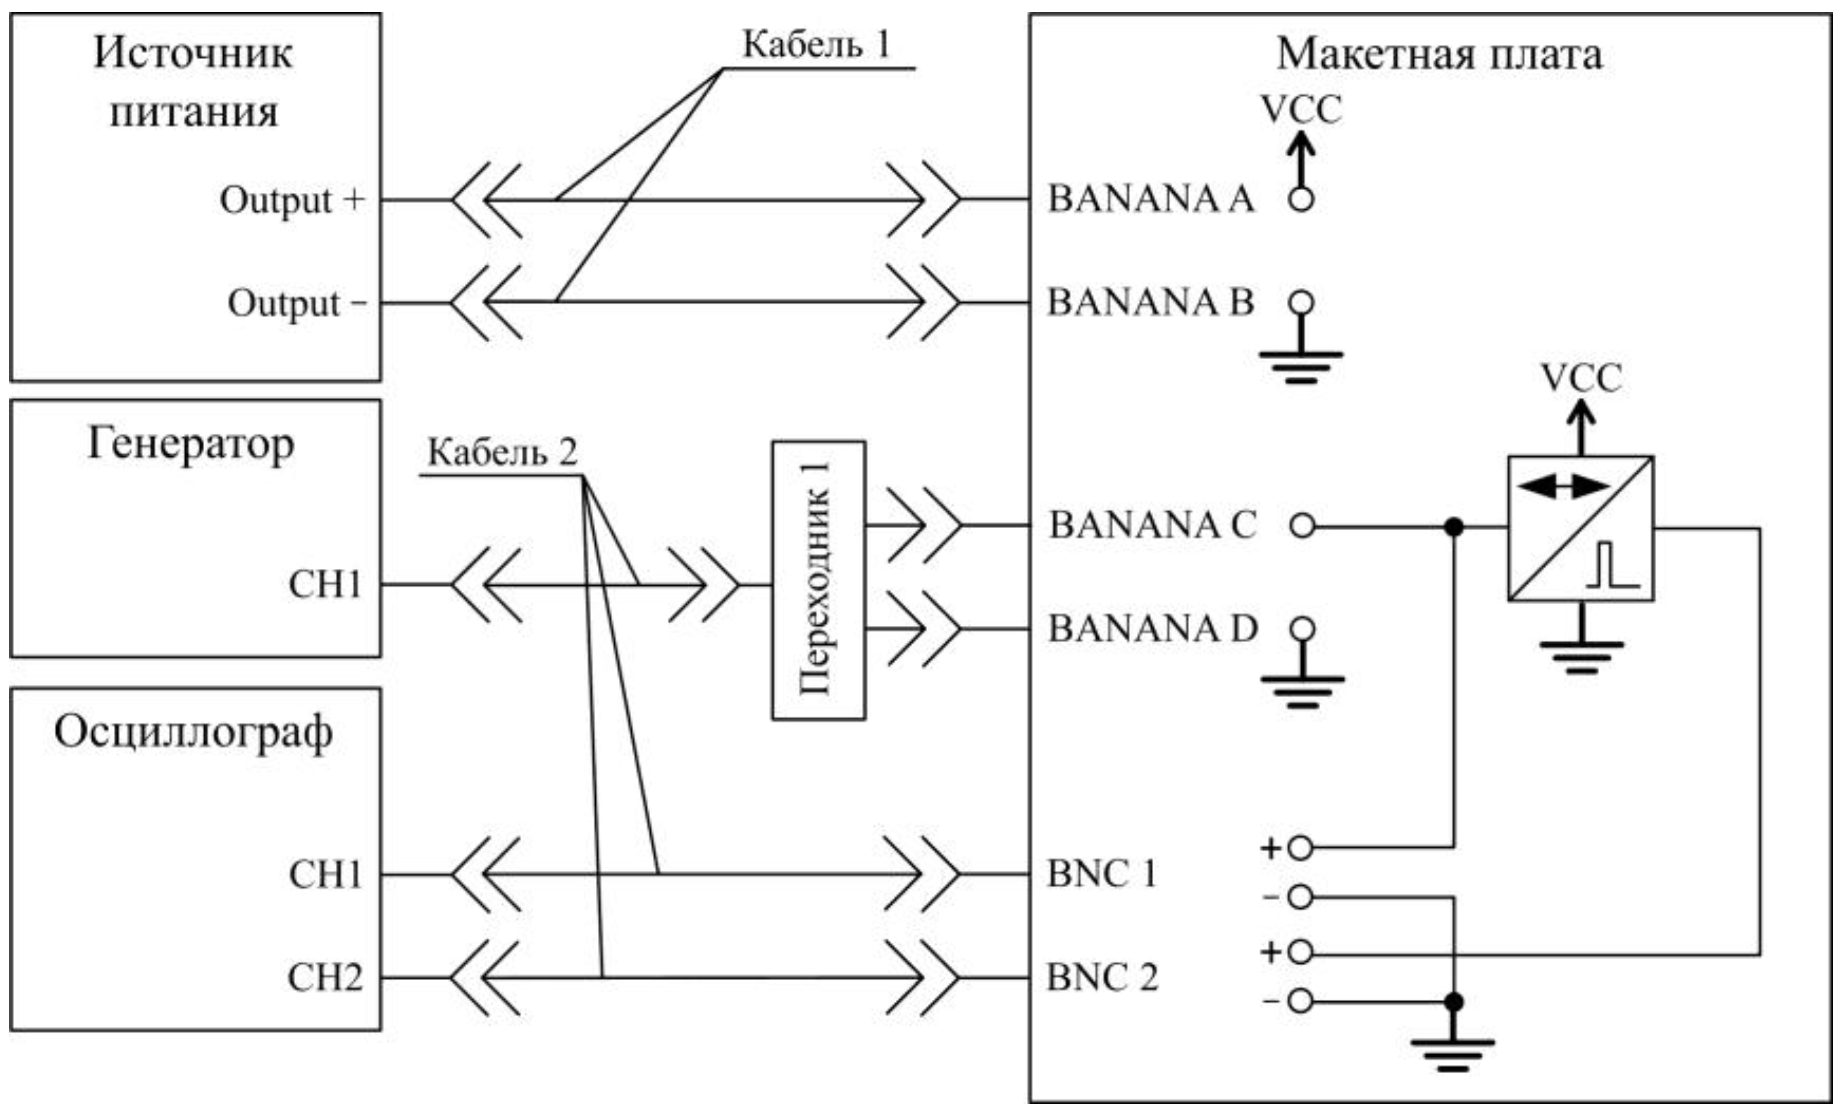
\includegraphics[width=\textwidth]{E1scheme.png}
	\caption{Схема для совместного измерения расстояния от дальномера до преграды и выходного параметра дальномера}
\end{figure}


\begin{table}[H]
\caption{Форма таблицы $A.4.1$ — Протокол совместного измерения расстояния от дальномера
до преграды и выходного параметра дальномера}
\label{tab:e1protocol}
\centering
\begin{tabularx}{\textwidth}{|p{0.5cm}|p{3cm}|p{3cm}|C|C|C|C|C|}
\hline
\multirow{2}{=}{\vspace{2em}\makecell[c]{\large\textsf{№}\\ п/п}} & \vspace{2em}\multirow{2}{=}{\centering Установленное расстояние, $D$, см} & \vspace{0.5em}\multirow{2}{=}{\centering Коэффициент горизонтальной развёртки осциллографа, мc/дел}\vspace{3em} & \multicolumn{5}{p{8cm}|}{\vspace{1em}\centering\makecell[c]{\large Измерения выходного \\ \large параметра дальномера, мс}} \\
\cline{4-8}
 & & & \raisebox{-1em}{$X_1$}\vspace{1em} & \raisebox{-1em}{$X_2$}\vspace{1em} & \raisebox{-1em}{$X_3$}\vspace{1em} & \raisebox{-1em}{$X_4$}\vspace{1em} & \raisebox{-1em}{$X_5$}\vspace{1em} \\
\hline
\directlua{print_e1_protocol()}
\end{tabularx}
\end{table}

Для первой строки таблицы \ref{tab:e1protocol1} среднее значение рассчитано по формуле \eqref{eq:mean-x}
\[
\begin{aligned}
\overline{X}_1 &=
\frac{1.1897 + 1.2167 + 1.2167 + 1.2166 + 1.2406}{5}
= \directlua{tex.sprint(value_with_mantice(E1[1].Xmean, 5, 0, 0))}\;\text{мс}
\end{aligned}
\]
Для той же строки стандартное отклонение рассчитано по формуле \eqref{eq:std-x}
\[
\begin{aligned}
S_{X_1} &=
\sqrt{
\begin{aligned}
  \frac{
  (1.1897 - \directlua{tex.sprint(value_with_mantice(E1[1].Xmean, 5, 0, 0))})^2 +
  (1.2167 - \directlua{tex.sprint(value_with_mantice(E1[1].Xmean, 5, 0, 0))})^2 +
  (1.2167 - \directlua{tex.sprint(value_with_mantice(E1[1].Xmean, 5, 0, 0))})^2 
  }{5 - 1}
  + \\ +
  \frac{
  (1.2166 - \directlua{tex.sprint(value_with_mantice(E1[1].Xmean, 5, 0, 0))})^2 +
  (1.2406 - \directlua{tex.sprint(value_with_mantice(E1[1].Xmean, 5, 0, 0))})^2}{5 - 1}
\end{aligned}
}
= \directlua{tex.sprint(value_with_mantice(E1[1].S, 3, -2, 0))}\;\text{мс}
\end{aligned}
\]

\begin{table}[H]
\caption{Значения среднего и стандартного отклонения для каждой точки градуировочной характеристики дальномера}
\label{tab:e1protocol1}
\centering
\begin{tabularx}{\textwidth}{|p{0.5cm}|p{3cm}|p{3cm}|C|C|}
\hline
\multirow{2}{=}{\vspace{2em}\makecell[c]{\large\textsf{№}\\ п/п}} & 
\vspace{2em}\multirow{2}{=}{\centering Установленное расстояние, $D$, см} & 
\vspace{0.5em}\multirow{2}{=}{\centering Коэффициент горизонтальной развёртки осциллографа, мc/дел}\vspace{3em} & 
\multicolumn{2}{p{8cm}|}{\vspace{1em}\centering\makecell[c]{\large Измерения выходного \\ \large параметра дальномера, мс}} \\
\cline{4-5}
 & & & \raisebox{-1em}{$X_\text{mean}$}\vspace{1em} & \raisebox{-1em}{$S$}\vspace{1em} \\
\hline
\directlua{print_e1_protocol1()}
\end{tabularx}
\end{table}

\subsection{Графический анализ исходных результатов измерений}

По исходным точкам видно, что при увеличении расстояния $D$ выходной
параметр дальномера $X$ монотонно возрастает. Форма облака точек вытянута
вдоль прямой линии, поэтому в качестве рабочей гипотезы принимается линейная
градуировочная характеристика.

\begin{table}[H]
\caption{Медианные центры для предварительного выбора модели}
\label{tab:e1median}
\begin{tabularx}{\textwidth}{|C|C|C|}
\hline
Группа & $D_{\text{мед}}$, см & $X_{\text{мед}}$, мс\\
\hline
\directlua{print_e1_median_centers()}
\end{tabularx}
\end{table}

Медианные центры в таблице \ref{tab:e1median} были рассчитаны для предварительного 
выбора вида аппроксимирующей функции. Медиана слабее среднего значения реагирует
на отдельные выбросы, поэтому взаимное расположение медианных центров
позволяет устойчиво проверить, вытянуто ли облако точек вдоль прямой.
Так как три медианных центра расположены почти линейно, далее используется
линейная модель \eqref{eq:linear-model}, а численные коэффициенты уже
уточняются методом наименьших квадратов.

\begin{figure}[H]
\centering
\begin{tikzpicture}
\begin{axis}[
    width=\textwidth,
    height=0.52\textwidth,
    grid=both,
    minor tick num=4,
    xlabel={$D$, см},
    ylabel={$X$, мс},
    xmin=15, xmax=105,
    ymin=1.0, ymax=6.1,
    legend pos=north west,
]
\addplot[only marks, mark=*, mark size=1.3pt] coordinates {\directlua{print_e1_all_points()}};
\addlegendentry{Исходные измерения}
\addplot[only marks, mark=square*, mark size=2.0pt] coordinates {\directlua{print_e1_mean_points()}};
\addlegendentry{Средние значения}
\addplot[only marks, mark=diamond*, mark size=2.4pt] coordinates {\directlua{print_e1_median_points()}};
\addlegendentry{Медианные центры}
\end{axis}
\end{tikzpicture}
\caption{Исходные результаты совместных измерений}
\label{fig:e1points}
\end{figure}

\subsection{Аппроксимация методом наименьших квадратов}

Для обработки всех экспериментальных точек была выбрана линейная модель \eqref{eq:linear-model}
\[
X = b_0 + b_1D
\]

Коэффициенты линейной модели вычисляются по формулам \eqref{eq:e1-b1} и \eqref{eq:e1-b0}, полученным из нормальных уравнений \eqref{eq:mnk-solution}

Коэффициент $b_1$ вычисляется по формуле \eqref{eq:e1-b1}
\[
\begin{aligned}
b_1 &=
\frac{
\directlua{tex.sprint(value_with_mantice(E1FIT.n, 3, 1, 0))}\cdot
\directlua{tex.sprint(value_with_mantice(E1FIT.sxy, 6, 4, 0))} -
\directlua{tex.sprint(value_with_mantice(E1FIT.sx, 5, 3, 0))}\cdot
\directlua{tex.sprint(value_with_mantice(E1FIT.sy, 6, 2, 0))}
}{
\directlua{tex.sprint(value_with_mantice(E1FIT.det, 6, 6, 0))}
}
= \directlua{tex.sprint(value_with_mantice(E1FIT.b1, 5, -2, 0))}\;\text{мс/см}
\end{aligned}
\]

Коэффициент $b_0$ вычисляется по формуле \eqref{eq:e1-b0}
\[
\begin{aligned}
b_0 &=
\frac{
\directlua{tex.sprint(value_with_mantice(E1FIT.sy, 6, 2, 0))} -
\directlua{tex.sprint(value_with_mantice(E1FIT.b1, 5, -2, 0))}\cdot
\directlua{tex.sprint(value_with_mantice(E1FIT.sx, 5, 3, 0))}
}{
\directlua{tex.sprint(value_with_mantice(E1FIT.n, 3, 1, 0))}
}
= \directlua{tex.sprint(value_with_mantice(E1FIT.b0, 5, -1, 0))}\;\text{мс}
\end{aligned}
\]

Следовательно, градуировочная характеристика дальномера имеет вид
\[
X = \directlua{tex.sprint(value_with_mantice(E1FIT.b0, 5, -1, 0))}
+ \directlua{tex.sprint(value_with_mantice(E1FIT.b1, 5, -2, 0))}D
\]

В обратной форме, если требуется определить расстояние по измеренной длительности,
получаем
\[
D = \frac{X - b_0}{b_1}
\]

Остаточная выборочная дисперсия вычислялась по формуле \eqref{eq:residual-variance}
\[
\begin{aligned}
S^2 &=
\frac{\directlua{tex.sprint(value_with_mantice(E1FIT.ss_res, 6, -1, 0))}}
{\directlua{tex.sprint(value_with_mantice(E1FIT.n, 3, 1, 0))} -
\directlua{tex.sprint(value_with_mantice(E1FIT.m, 3, 0, 0))}}
= \directlua{tex.sprint(value_with_mantice(E1FIT.S2, 5, -3, 0))}\;\text{мс}^2\\
S &= \sqrt{\directlua{tex.sprint(value_with_mantice(E1FIT.S2, 5, -3, 0))}}
= \directlua{tex.sprint(value_with_mantice(E1FIT.S, 5, -2, 0))}\;\text{мс}
\end{aligned}
\]

\subsection{Доверительные границы коэффициентов}

Число экспериментальных значений равно
\[
n = \directlua{tex.sprint(value_with_mantice(E1FIT.n, 3, 1, 0))}
\]
а число степеней свободы для линейной модели
\[
\nu = n - 2 =
\directlua{tex.sprint(value_with_mantice(E1FIT.n, 3, 1, 0))} -
\directlua{tex.sprint(value_with_mantice(E1FIT.m, 3, 0, 0))}
= \directlua{tex.sprint(value_with_mantice(E1FIT.df, 3, 1, 0))}
\]
Для доверительной вероятности $0.95$ был использован квантиль
\[
t_{0.05;\,\nu} = \directlua{tex.sprint(value_with_mantice(E1FIT.t, 5, 0, 0))}
\]

Диагональные элементы ковариационной матрицы вычислялись по формуле \eqref{eq:e1-v00}
\[
\begin{aligned}
V_{00} &=
\directlua{tex.sprint(value_with_mantice(E1FIT.S2, 5, -3, 0))}\cdot
\frac{\directlua{tex.sprint(value_with_mantice(E1FIT.sxx, 6, 5, 0))}}
{\directlua{tex.sprint(value_with_mantice(E1FIT.det, 6, 6, 0))}}
= \directlua{tex.sprint(value_with_mantice(E1FIT.V00, 5, -4, 0))}\\
V_{11} &=
\directlua{tex.sprint(value_with_mantice(E1FIT.S2, 5, -3, 0))}\cdot
\frac{\directlua{tex.sprint(value_with_mantice(E1FIT.n, 3, 1, 0))}}
{\directlua{tex.sprint(value_with_mantice(E1FIT.det, 6, 6, 0))}}
= \directlua{tex.sprint(value_with_mantice(E1FIT.V11, 5, -8, 0))}
\end{aligned}
\]

Погрешности коэффициентов вычислялись по формуле \eqref{eq:delta-coeff}
\[
\begin{aligned}
\Delta b_0 &=
\directlua{tex.sprint(value_with_mantice(E1FIT.t, 5, 0, 0))}\sqrt{
\directlua{tex.sprint(value_with_mantice(E1FIT.V00, 5, -4, 0))}}
= \directlua{tex.sprint(value_with_mantice(E1FIT.db0, 5, -2, 0))}\;\text{мс}\\
\Delta b_1 &=
\directlua{tex.sprint(value_with_mantice(E1FIT.t, 5, 0, 0))}\sqrt{
\directlua{tex.sprint(value_with_mantice(E1FIT.V11, 5, -8, 0))}}
= \directlua{tex.sprint(value_with_mantice(E1FIT.db1, 5, -4, 0))}\;\text{мс/см}
\end{aligned}
\]

Доверительные границы коэффициентов градуировочной характеристики вычислялись по формуле \eqref{eq:confidence-coeff}
\[
\begin{aligned}
b_0 &= \left(\directlua{tex.sprint(value_with_mantice(E1FIT.b0, 5, -1, 0))}
\pm \directlua{tex.sprint(value_with_mantice(E1FIT.db0, 5, -2, 0))}\right)\;\text{мс}\\
b_1 &= \left(\directlua{tex.sprint(value_with_mantice(E1FIT.b1, 5, -2, 0))}
\pm \directlua{tex.sprint(value_with_mantice(E1FIT.db1, 5, -4, 0))}\right)\;\text{мс/см}
\end{aligned}
\]

\begin{figure}[H]
\centering
\begin{tikzpicture}
\begin{axis}[
    width=\textwidth,
    height=0.52\textwidth,
    grid=both,
    minor tick num=4,
    xlabel={$D$, см},
    ylabel={$X$, мс},
    xmin=15, xmax=105,
    ymin=1.0, ymax=6.1,
    legend pos=north west,
]
\addplot[only marks, mark=*, mark size=1.3pt] coordinates {\directlua{print_e1_all_points()}};
\addlegendentry{Измерения}
\addplot[only marks, mark=diamond*, mark size=2.4pt] coordinates {\directlua{print_e1_median_points()}};
\addlegendentry{Медианные центры}
\addplot[domain=20:100, samples=2, thick] {\directlua{tex.sprint(raw_number(E1FIT.b0))} + \directlua{tex.sprint(raw_number(E1FIT.b1))} * x};
\addlegendentry{МНК}
\addplot[domain=20:100, samples=2, dashed] {\directlua{tex.sprint(raw_number(E1FIT.b0 + E1FIT.db0))} + \directlua{tex.sprint(raw_number(E1FIT.b1 + E1FIT.db1))} * x};
\addlegendentry{Верхняя доверительная граница}
\addplot[domain=20:100, samples=2, dashed] {\directlua{tex.sprint(raw_number(E1FIT.b0 - E1FIT.db0))} + \directlua{tex.sprint(raw_number(E1FIT.b1 - E1FIT.db1))} * x};
\addlegendentry{Нижняя доверительная граница}
\end{axis}
\end{tikzpicture}
\caption{Аппроксимация результатов совместных измерений с доверительными границами}
\label{fig:e1fit}
\end{figure}

\subsection{Оценка качества аппроксимации}

Коэффициент корреляции Пирсона для зависимости $X = f(D)$ вычислялся по формуле \eqref{eq:pearson} и равен
\begin{equation*}
\rho_{DX} = \directlua{tex.sprint(value_with_mantice(E1FIT.r, 6, -1, 0))} > \alpha = 0.95
\end{equation*}
Коэффициент детерминации вычислялся по формуле \eqref{eq:determination}, коэффициент 
множественной корреляции по формуле \eqref{eq:multiple-correlation}
\begin{equation*}
\begin{aligned}
R^2 &= \directlua{tex.sprint(value_with_mantice(E1FIT.R2, 6, -1, 0))} \\
\rho_{X\widehat{X}} &= \directlua{tex.sprint(value_with_mantice(E1FIT.rho, 6, -1, 0))} > \alpha = 0.95
\end{aligned}
\end{equation*}

Линейная условная функция выбрана верно. Остаточное отклонение мало
по сравнению с диапазоном изменения выходного параметра дальномера, поэтому
полученная градуировочная характеристика пригодна для оценки расстояния
по измеренному выходному параметру.

\fancyhead[L]{Задание $2$}
\section{Совокупные измерения для оценки сопротивлений $R_1$, $R_2$, $R_3$}

\subsection{Схема и протокол совокупных измерений}

Для разных значений напряжения питания измерялись ток потребления цепи и напряжения
в точках A и B. 

\begin{figure}[H]
	\centering
	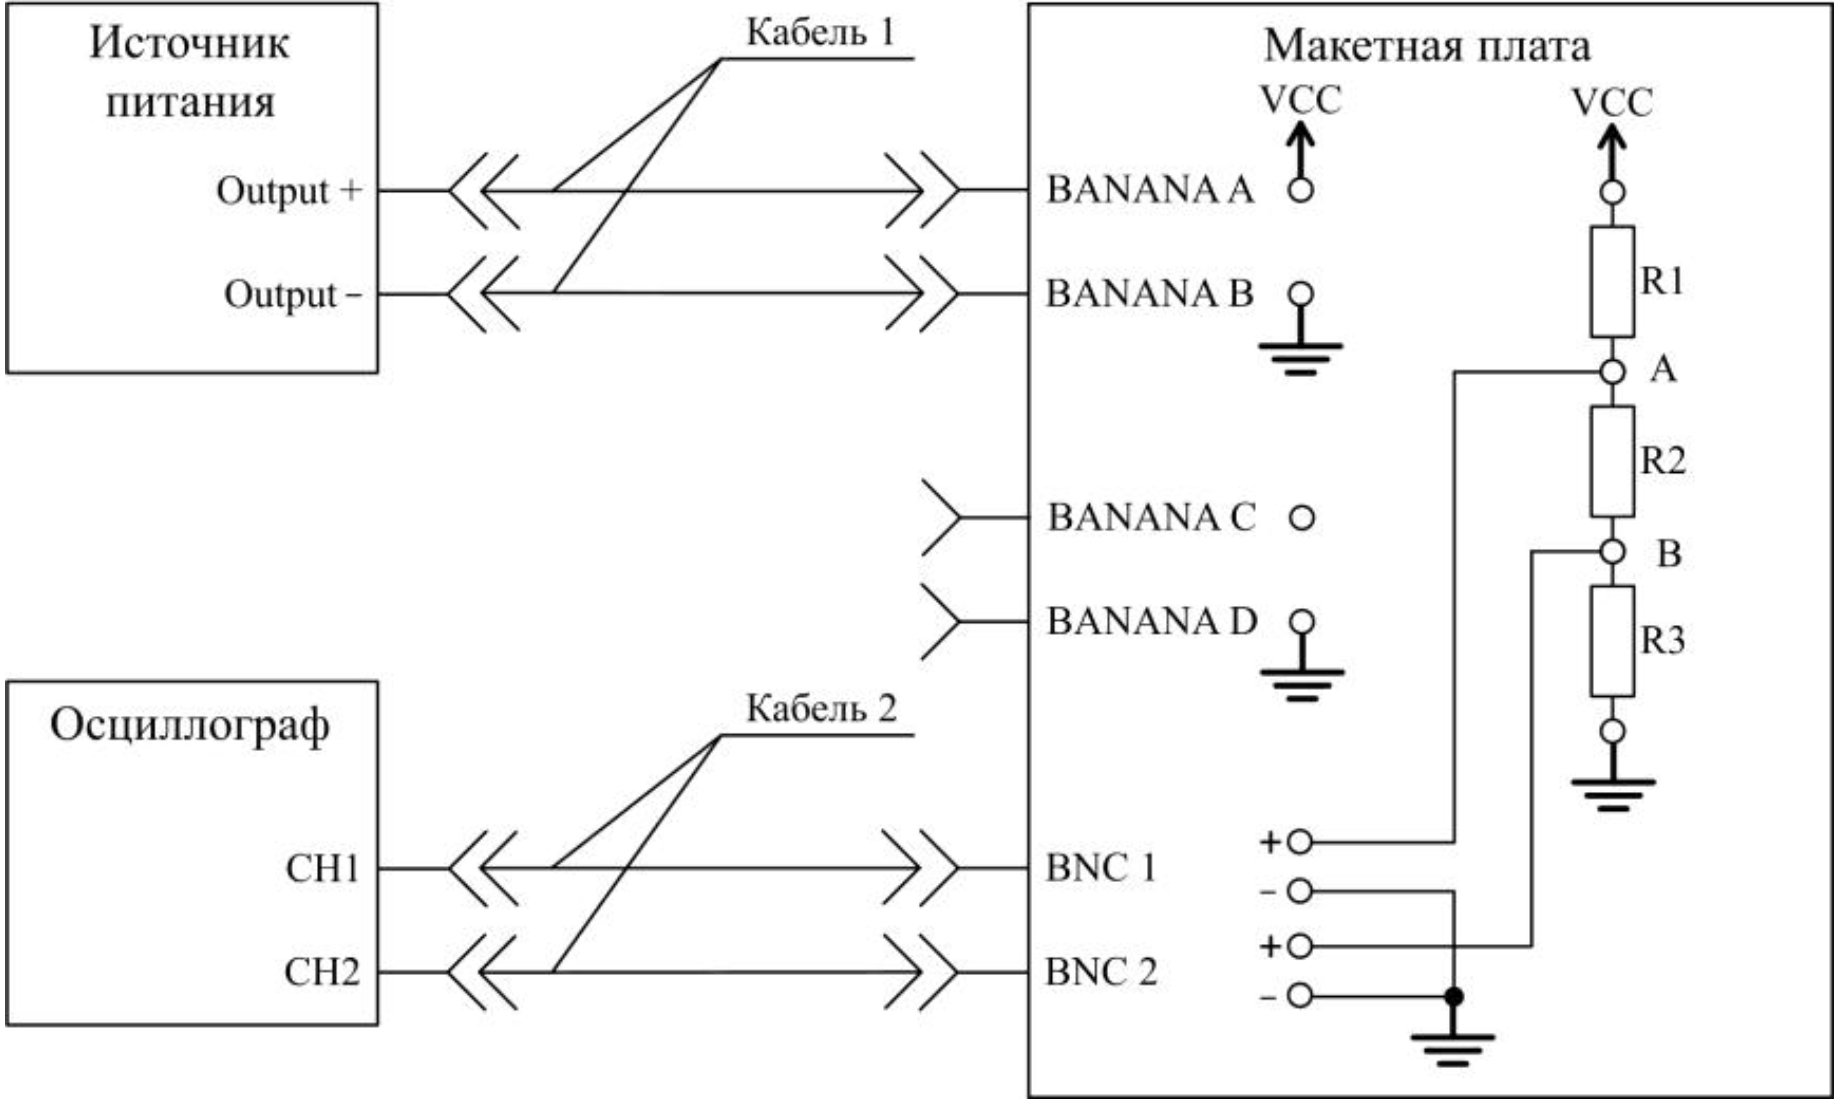
\includegraphics[width=\textwidth]{E2scheme.png}
	\caption{Схема совокупных измерений сопротивлений $R_1$, $R_2$, $R_3$}
\end{figure}


\begin{table}[H]
\caption{Форма таблицы A$.4.2$ – Протокол совокупных измерений напряжения
питания цепи, тока потребления схемы и падений напряжений
в точках A и B}
\label{tab:e2protocol}
\begin{tabularx}{\textwidth}{|p{0.5cm}|C|C|C|C|}
\hline
\multirow{2}{=}{\textsf{№}} & \multicolumn{2}{p{7cm}|}{ \centering Показания источника питания } & \multicolumn{2}{p{7cm}|}{ \centering Измеренные напряжения } \\
\cline{2-5}
 & Напряжение питания схемы, В & Ток потребления схемы, А & Измеренное напряжение в точке A, В & Измеренное напряжение в точке B, В\\
\hline
\directlua{print_e2_protocol()}
\end{tabularx}
\end{table}

По измеренным значениям из таблицы \ref{tab:e2protocol} падения
напряжений на участках цепи были найдены по формуле \eqref{eq:e2-drops}
\begin{equation}
U_{R_1} = U_{\text{пит}} - U_A\qquad
U_{R_2} = U_A - U_B\qquad
U_{R_3} = U_B
\tag{8.1}
\label{eq:e2-drops}
\end{equation}

Для первой строки протокола падения напряжений рассчитаны по формуле \eqref{eq:e2-drops}
\[
\begin{aligned}
U_{R_1,1} &= 0.999 - 0.73341
= \directlua{tex.sprint(value_with_mantice(E2[1].U - E2[1].UA, 5, -1, 0))}\;\text{В}\\
U_{R_2,1} &= 0.73341 - 0.42816
= \directlua{tex.sprint(value_with_mantice(E2[1].UA - E2[1].UB, 5, -1, 0))}\;\text{В}\\
U_{R_3,1} &= 0.42816
= \directlua{tex.sprint(value_with_mantice(E2[1].UB, 5, -1, 0))}\;\text{В}
\end{aligned}
\]

\begin{table}[H]
\caption{Падения напряжений, используемые при составлении системы уравнений}
\label{tab:e2drops}
\begin{tabularx}{\textwidth}{|p{0.5cm}|C|C|C|}
\hline
\textsf{№} & $U_{R_1}$, В & $U_{R_2}$, В & $U_{R_3}$, В \vspace{0.2em}\\
\hline
\directlua{print_e2_drop_table()}
\end{tabularx}
\end{table}

\subsection{Система уравнений для оценки сопротивлений}

Для каждой строки протокола записывается система
\begin{equation*}
\begin{cases}
I_iR_1 = U_{\text{пит},i} - U_{A,i} \\
I_iR_2 = U_{A,i} - U_{B,i} \\
I_iR_3 = U_{B,i}
\end{cases}
\end{equation*}

Для первой строки протокола она имеет вид
\begin{equation*}
\begin{cases}
\directlua{tex.sprint(value_with_mantice(E2[1].I, 4, -3, 0))}R_1
= \directlua{tex.sprint(value_with_mantice(E2[1].U, 4, -1, 0))}
- \directlua{tex.sprint(value_with_mantice(E2[1].UA, 5, -1, 0))} \\
\directlua{tex.sprint(value_with_mantice(E2[1].I, 4, -3, 0))}R_2
= \directlua{tex.sprint(value_with_mantice(E2[1].UA, 5, -1, 0))}
- \directlua{tex.sprint(value_with_mantice(E2[1].UB, 5, -1, 0))} \\
\directlua{tex.sprint(value_with_mantice(E2[1].I, 4, -3, 0))}R_3
= \directlua{tex.sprint(value_with_mantice(E2[1].UB, 5, -1, 0))}
\end{cases}
\end{equation*}
После вычисления разностей напряжений
\begin{equation*}
\begin{cases}
\directlua{tex.sprint(value_with_mantice(E2[1].I, 4, -3, 0))}R_1
= \directlua{tex.sprint(value_with_mantice(E2[1].U - E2[1].UA, 5, -1, 0))}\\
\directlua{tex.sprint(value_with_mantice(E2[1].I, 4, -3, 0))}R_2
= \directlua{tex.sprint(value_with_mantice(E2[1].UA - E2[1].UB, 5, -1, 0))}\\
\directlua{tex.sprint(value_with_mantice(E2[1].I, 4, -3, 0))}R_3
= \directlua{tex.sprint(value_with_mantice(E2[1].UB, 5, -1, 0))}
\end{cases}
\end{equation*}

Для всех строк таблицы система записывается в матричном виде
\begin{equation*}
\begin{pmatrix}
I_1 & 0 & 0\\
0 & I_1 & 0\\
0 & 0 & I_1\\
I_2 & 0 & 0\\
0 & I_2 & 0\\
0 & 0 & I_2\\
\ldots & \ldots & \ldots
\end{pmatrix}
\begin{pmatrix}
R_1\\R_2\\R_3
\end{pmatrix}
=
\begin{pmatrix}
U_{\text{пит},1} - U_{A,1}\\
U_{A,1} - U_{B,1}\\
U_{B,1}\\
U_{\text{пит},2} - U_{A,2}\\
U_{A,2} - U_{B,2}\\
U_{B,2}\\
\ldots
\end{pmatrix}
\end{equation*}

\subsection{Решение системы методом наименьших квадратов}

Значения сопротивлений были найдены по формуле \eqref{eq:mnk-resistors}
\[
\mathbf{R} = \left(X^TX\right)^{-1}X^T\mathbf{y}
\]
Для данной структуры системы используется эквивалентная расчетная форма
\eqref{eq:resistor-simple}.

Сопротивление $R_1$ вычисляется по формуле \eqref{eq:resistor-simple}
\[
\begin{aligned}
R_1 &=
\frac{\sum I_iU_{R_1,i}}{\sum I_i^2}
=
\frac{\directlua{tex.sprint(value_with_mantice(E2FIT.sumIR1, 6, -2, 0))}}
{\directlua{tex.sprint(value_with_mantice(E2FIT.sumI2, 5, -5, 0))}}
= \directlua{tex.sprint(value_with_mantice(E2FIT.R1, 5, 2, 0))}\;\text{Ом}
\end{aligned}
\]

Сопротивление $R_2$ вычисляется по формуле \eqref{eq:resistor-simple}
\[
\begin{aligned}
R_2 &=
\frac{\sum I_iU_{R_2,i}}{\sum I_i^2}
=
\frac{\directlua{tex.sprint(value_with_mantice(E2FIT.sumIR2, 6, -2, 0))}}
{\directlua{tex.sprint(value_with_mantice(E2FIT.sumI2, 5, -5, 0))}}
= \directlua{tex.sprint(value_with_mantice(E2FIT.R2, 5, 2, 0))}\;\text{Ом}
\end{aligned}
\]

Сопротивление $R_3$ вычисляется по формуле \eqref{eq:resistor-simple}
\[
\begin{aligned}
R_3 &=
\frac{\sum I_iU_{R_3,i}}{\sum I_i^2}
=
\frac{\directlua{tex.sprint(value_with_mantice(E2FIT.sumIR3, 6, -2, 0))}}
{\directlua{tex.sprint(value_with_mantice(E2FIT.sumI2, 5, -5, 0))}}
= \directlua{tex.sprint(value_with_mantice(E2FIT.R3, 5, 2, 0))}\;\text{Ом}
\end{aligned}
\]

Для проверки результата на графике строятся экспериментальные зависимости
$U_{R_j} = f(I)$ и прямые аппроксимации
\[
U_{R_1} = R_1I\qquad U_{R_2} = R_2I\qquad U_{R_3} = R_3I
\]

\begin{figure}[H]
\centering
\begin{tikzpicture}
\begin{axis}[
    width=\textwidth,
    height=0.58\textwidth,
    grid=both,
    minor tick num=4,
    xlabel={$I$, мА},
    ylabel={$U_R$, В},
    xmin=0, xmax=6.5,
    ymin=0, ymax=5.2,
    legend pos=north west,
]
\addplot[only marks, mark=*, mark size=1.3pt] coordinates {\directlua{print_e2_ur_points(1)}};
\addlegendentry{$U_{R_1}$}
\addplot[domain=0:6.2, samples=2, thick] {\directlua{tex.sprint(raw_number(E2FIT.R1 / 1000))} * x};
\addlegendentry{$R_1I$}
\addplot[domain=0:6.2, samples=2, dashed] {\directlua{tex.sprint(raw_number((E2FIT.R1 + E2FIT.dR1) / 1000))} * x};
\addlegendentry{$(R_1+\Delta R_1)I$}
\addplot[domain=0:6.2, samples=2, dashed] {\directlua{tex.sprint(raw_number((E2FIT.R1 - E2FIT.dR1) / 1000))} * x};
\addlegendentry{$(R_1-\Delta R_1)I$}
\addplot[only marks, mark=square*, mark size=1.3pt] coordinates {\directlua{print_e2_ur_points(2)}};
\addlegendentry{$U_{R_2}$}
\addplot[domain=0:6.2, samples=2, thick] {\directlua{tex.sprint(raw_number(E2FIT.R2 / 1000))} * x};
\addlegendentry{$R_2I$}
\addplot[domain=0:6.2, samples=2, dashed, forget plot] {\directlua{tex.sprint(raw_number((E2FIT.R2 + E2FIT.dR2) / 1000))} * x};
\addplot[domain=0:6.2, samples=2, dashed, forget plot] {\directlua{tex.sprint(raw_number((E2FIT.R2 - E2FIT.dR2) / 1000))} * x};
\addplot[only marks, mark=triangle*, mark size=1.5pt] coordinates {\directlua{print_e2_ur_points(3)}};
\addlegendentry{$U_{R_3}$}
\addplot[domain=0:6.2, samples=2, thick] {\directlua{tex.sprint(raw_number(E2FIT.R3 / 1000))} * x};
\addlegendentry{$R_3I$}
\addplot[domain=0:6.2, samples=2, dashed, forget plot] {\directlua{tex.sprint(raw_number((E2FIT.R3 + E2FIT.dR3) / 1000))} * x};
\addplot[domain=0:6.2, samples=2, dashed, forget plot] {\directlua{tex.sprint(raw_number((E2FIT.R3 - E2FIT.dR3) / 1000))} * x};
\end{axis}
\end{tikzpicture}
\caption{Аппроксимация зависимостей падений напряжения на резисторах от тока с доверительными границами}
\label{fig:e2fit}
\end{figure}

Линейная аппроксимация экспериментальных точек недостаточно хорошо описывает их поведение, но 
выбрана для физической согласованности. 

Остаточная выборочная дисперсия для совокупных измерений вычислялась по формуле 
\eqref{eq:residual-variance}
\[
\begin{aligned}
S^2 &=
\frac{\directlua{tex.sprint(value_with_mantice(E2FIT.ss, 6, 0, 0))}}
{\directlua{tex.sprint(value_with_mantice(E2FIT.n, 3, 1, 0))} -
\directlua{tex.sprint(value_with_mantice(E2FIT.m, 3, 0, 0))}}
= \directlua{tex.sprint(value_with_mantice(E2FIT.S2, 5, -1, 0))}\;\text{В}^2\\
S &= \sqrt{\directlua{tex.sprint(value_with_mantice(E2FIT.S2, 5, -1, 0))}}
= \directlua{tex.sprint(value_with_mantice(E2FIT.S, 5, -1, 0))}\;\text{В}
\end{aligned}
\]

Число уравнений равно
\[
n = \directlua{tex.sprint(value_with_mantice(E2FIT.n, 3, 1, 0))}
\]
число неизвестных равно $m = 3$, поэтому число степеней свободы
\[
\nu = n - m =
\directlua{tex.sprint(value_with_mantice(E2FIT.n, 3, 1, 0))} -
\directlua{tex.sprint(value_with_mantice(E2FIT.m, 3, 0, 0))}
= \directlua{tex.sprint(value_with_mantice(E2FIT.df, 3, 1, 0))}
\]
Для доверительной вероятности $0,95$ использован квантиль
\[
t_{0.05;\,\nu} = \directlua{tex.sprint(value_with_mantice(E2FIT.t, 5, 0, 0))}
\]

В соответствии с формулой \eqref{eq:covariance} для каждого сопротивления
\[
V_{R_j} =
\frac{S^2}{\sum I_i^2}
=
\frac{\directlua{tex.sprint(value_with_mantice(E2FIT.S2, 5, -1, 0))}}
{\directlua{tex.sprint(value_with_mantice(E2FIT.sumI2, 5, -5, 0))}}
= \directlua{tex.sprint(value_with_mantice(E2FIT.V, 5, 3, 0))}\;\text{Ом}^2
\]

Погрешность сопротивления для доверительной вероятности $0,95$ вычислялась по формуле \eqref{eq:confidence-coeff}
\[
\Delta R_j =
\directlua{tex.sprint(value_with_mantice(E2FIT.t, 5, 0, 0))}\sqrt{
\directlua{tex.sprint(value_with_mantice(E2FIT.V, 5, 3, 0))}}
= \directlua{tex.sprint(value_with_mantice(E2FIT.dR1, 5, 1, 0))}\;\text{Ом}
\]

Итоговые значения сопротивлений с 95\%-ными доверительными границами, вычисленными по формуле \eqref{eq:confidence-coeff}
\[
\begin{aligned}
R_1 &= \left(\directlua{tex.sprint(value_with_mantice(E2FIT.R1, 3, 2, 0))}
\pm \directlua{tex.sprint(value_with_mantice(E2FIT.dR1, 2, 1, 0))}\right)\;\text{Ом}\\
R_2 &= \left(\directlua{tex.sprint(value_with_mantice(E2FIT.R2, 3, 2, 0))}
\pm \directlua{tex.sprint(value_with_mantice(E2FIT.dR2, 2, 1, 0))}\right)\;\text{Ом}\\
R_3 &= \left(\directlua{tex.sprint(value_with_mantice(E2FIT.R3, 3, 2, 0))}
\pm \directlua{tex.sprint(value_with_mantice(E2FIT.dR3, 2, 1, 0))}\right)\;\text{Ом}
\end{aligned}
\]

\fancyhead[L]{Выводы}
\section{Выводы}

В ходе лабораторной работы была достигнута цель работы: были выполнены
многократные совместные измерения и совокупные измерения, после чего
действительные значения измеряемых величин были оценены методом наименьших
квадратов с последующей оценкой погрешностей полученных результатов.

В первой части работы была получена градуировочная характеристика
ультразвукового дальномера. По исходным экспериментальным точкам и методу
медианных центров была выбрана линейная модель зависимости выходного
параметра дальномера от расстояния до преграды. Методом наименьших квадратов
по формуле \eqref{eq:linear-model} получена зависимость
\begin{equation*}
X = \directlua{tex.sprint(value_with_mantice(E1FIT.b0, 5, -1, 0))}
+ \directlua{tex.sprint(value_with_mantice(E1FIT.b1, 5, -2, 0))}D
\end{equation*}
где $X$ выражается в миллисекундах, а $D$ – в сантиметрах. Коэффициенты
градуировочной характеристики с $95$\%-ными доверительными границами, вычисленными по формуле \eqref{eq:confidence-coeff}, равны
\begin{equation*}
\begin{aligned}
b_0 &= \left(\directlua{tex.sprint(value_with_mantice(E1FIT.b0, 3, -1, 0))}
\pm \directlua{tex.sprint(value_with_mantice(E1FIT.db0, 2, -2, 0))}\right)\;\text{мс} \\
b_1 &= \left(\directlua{tex.sprint(value_with_mantice(E1FIT.b1, 4, -2, 0))}
\pm \directlua{tex.sprint(value_with_mantice(E1FIT.db1, 2, -4, 0))}\right)\;\text{мс/см}
\end{aligned}
\end{equation*}
Коэффициент корреляции Пирсона составил
$\rho_{DX} = \directlua{tex.sprint(value_with_mantice(E1FIT.r, 6, -1, 0))}$,
а коэффициент множественной корреляции
$\rho_{X\widehat{X}} = \directlua{tex.sprint(value_with_mantice(E1FIT.rho, 6, -1, 0))}$.
Так как оба коэффициента больше $0.95$, выбранная линейная модель корректно
описывает экспериментальные данные в пределах полученной погрешности.

Во второй части работы были выполнены совокупные измерения для оценки
сопротивлений $R_1$, $R_2$ и $R_3$. По измеренным значениям напряжения
питания, тока потребления и напряжений в точках A и B была составлена
переопределенная система уравнений, решенная методом наименьших квадратов по формуле \eqref{eq:mnk-resistors}.
Получены следующие значения сопротивлений с $95$\%-ными доверительными
границами:
\begin{equation*}
\begin{aligned}
R_1 &= \left(\directlua{tex.sprint(value_with_mantice(E2FIT.R1, 3, 2, 0))}
\pm \directlua{tex.sprint(value_with_mantice(E2FIT.dR1, 2, 1, 0))}\right)\;\text{Ом} \\
R_2 &= \left(\directlua{tex.sprint(value_with_mantice(E2FIT.R2, 3, 2, 0))}
\pm \directlua{tex.sprint(value_with_mantice(E2FIT.dR2, 2, 1, 0))}\right)\;\text{Ом} \\
R_3 &= \left(\directlua{tex.sprint(value_with_mantice(E2FIT.R3, 3, 2, 0))}
\pm \directlua{tex.sprint(value_with_mantice(E2FIT.dR3, 2, 1, 0))}\right)\;\text{Ом}
\end{aligned}
\end{equation*}
Полученные значения сопротивлений согласуются с характером изменения
напряжений в точках A и B при изменении напряжения питания: при увеличении
$U_{\text{пит}}$ напряжения $U_A$ и $U_B$ возрастают почти пропорционально,
что соответствует резистивной цепи с постоянными параметрами.

\pagebreak
\fancyhead[L]{Список литературы}
\fancyhead[R]{\LabTitle}

\section*{Список использованной литературы}
\addcontentsline{toc}{section}{Список использованной литературы}

\begin{enumerate}
\item Калеев Д. В. \textit{Метрология и электрорадиоизмерения: лабораторный практикум}. М.: МИЭТ, 2025. 184 с.
\item RIGOL. \textit{Руководство по эксплуатации цифровых мультиметров DM3068, DM3058, DM3058E}. 2019.
\item RIGOL. \textit{Руководство по эксплуатации генераторов функций/сигналов произвольной формы серии DG1000Z}. 2019.
\item RIGOL. \textit{Руководство по эксплуатации цифрового осциллографа серии MSO5000}. 2019.
\item RIGOL. \textit{Руководство пользователя программируемого линейного источника питания серии DP800A}. 2012.
\end{enumerate}

\end{document}
